\documentclass[fleqn,10pt]{olplainarticle}
% Use option lineno for line numbers 

\title{Height Estimation using Numerical Methods and Kalman Filter}
\author[1]{Sensor Systems - Project 2\\Rikke Winberg - 1061864}


\begin{abstract}
The aim of this project is 
\end{abstract}

\begin{document}

\flushbottom
\maketitle
\thispagestyle{empty}




\section{Calibration of Pressure Sensor}


VIS LIGNING FOR HVORDAN HØJDEN REGNES FRA TRYK MÅLINGERNE
 
\section{Part 1 - Estimation of Velocity and Distance}

Data from the accelerometer and pressure sensor is collected where the sensors are raised up two meters and down again to the starting point. The data is imported into Matlab.\\

The gravity is accounted for in the accelerometer data by offsetting it such that the acceleration is 0 when the sensor is stationary. The acceleration, $\ddot{x}$, is integrated to get the vertical velocity, $\dot{x}$, in equation \ref{eq_acc_to_vel}.

\begin{align}
    \dot{x}_k = \dot{x}_{k-1} + \ddot{x}_k \, (t_k - t_{k-1})
    \label{eq_acc_to_vel}
\end{align}

The calculated velocities are integrated to get the vertical distance, $x_{acc}$, in equation \ref{eq_vel_to_pos}.

\begin{align}
    x_{k} = x_{k-1} + \dot{x}_{k} \, (t_{k} - t_{k-1})
    \label{eq_vel_to_pos}
\end{align}

 The pressure from the pressure sensor is used to calculate the height by the following equation KILDE:

\begin{align}
    x = 44330 \, \left[ 1 - \left( \frac{p}{p_0} \right)^{0.19} \right] \, \textit{m}
\end{align}

double integrator: bode diagram. error off set adds up. smoothens out graph.

differentiator: bode digram. error not a problem, graph is noisy.


\begin{figure}[H]
\centering
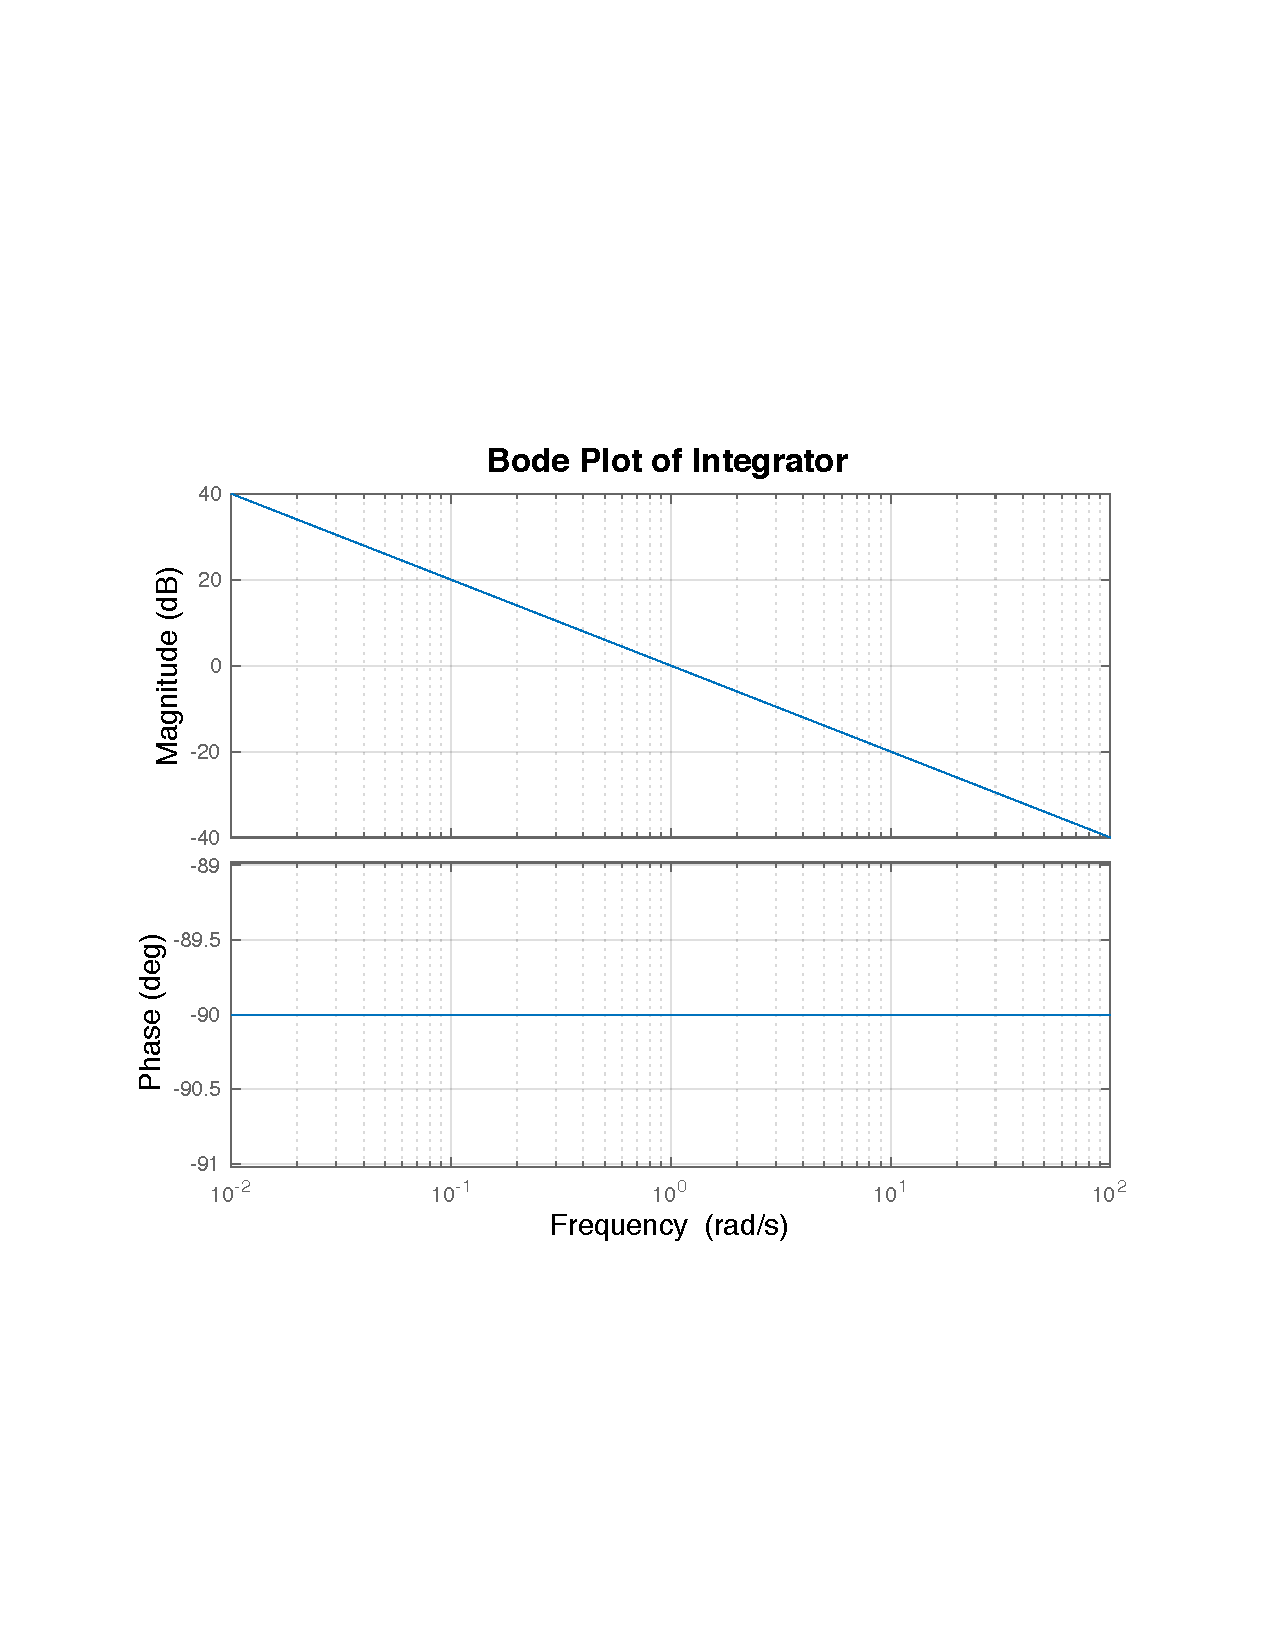
\includegraphics[width=0.8\linewidth]{figures/Integrator.pdf}
\caption{Bode plot of integrator.}
\label{fig_bode_integrator}
\end{figure}

\begin{figure}[H]
\centering
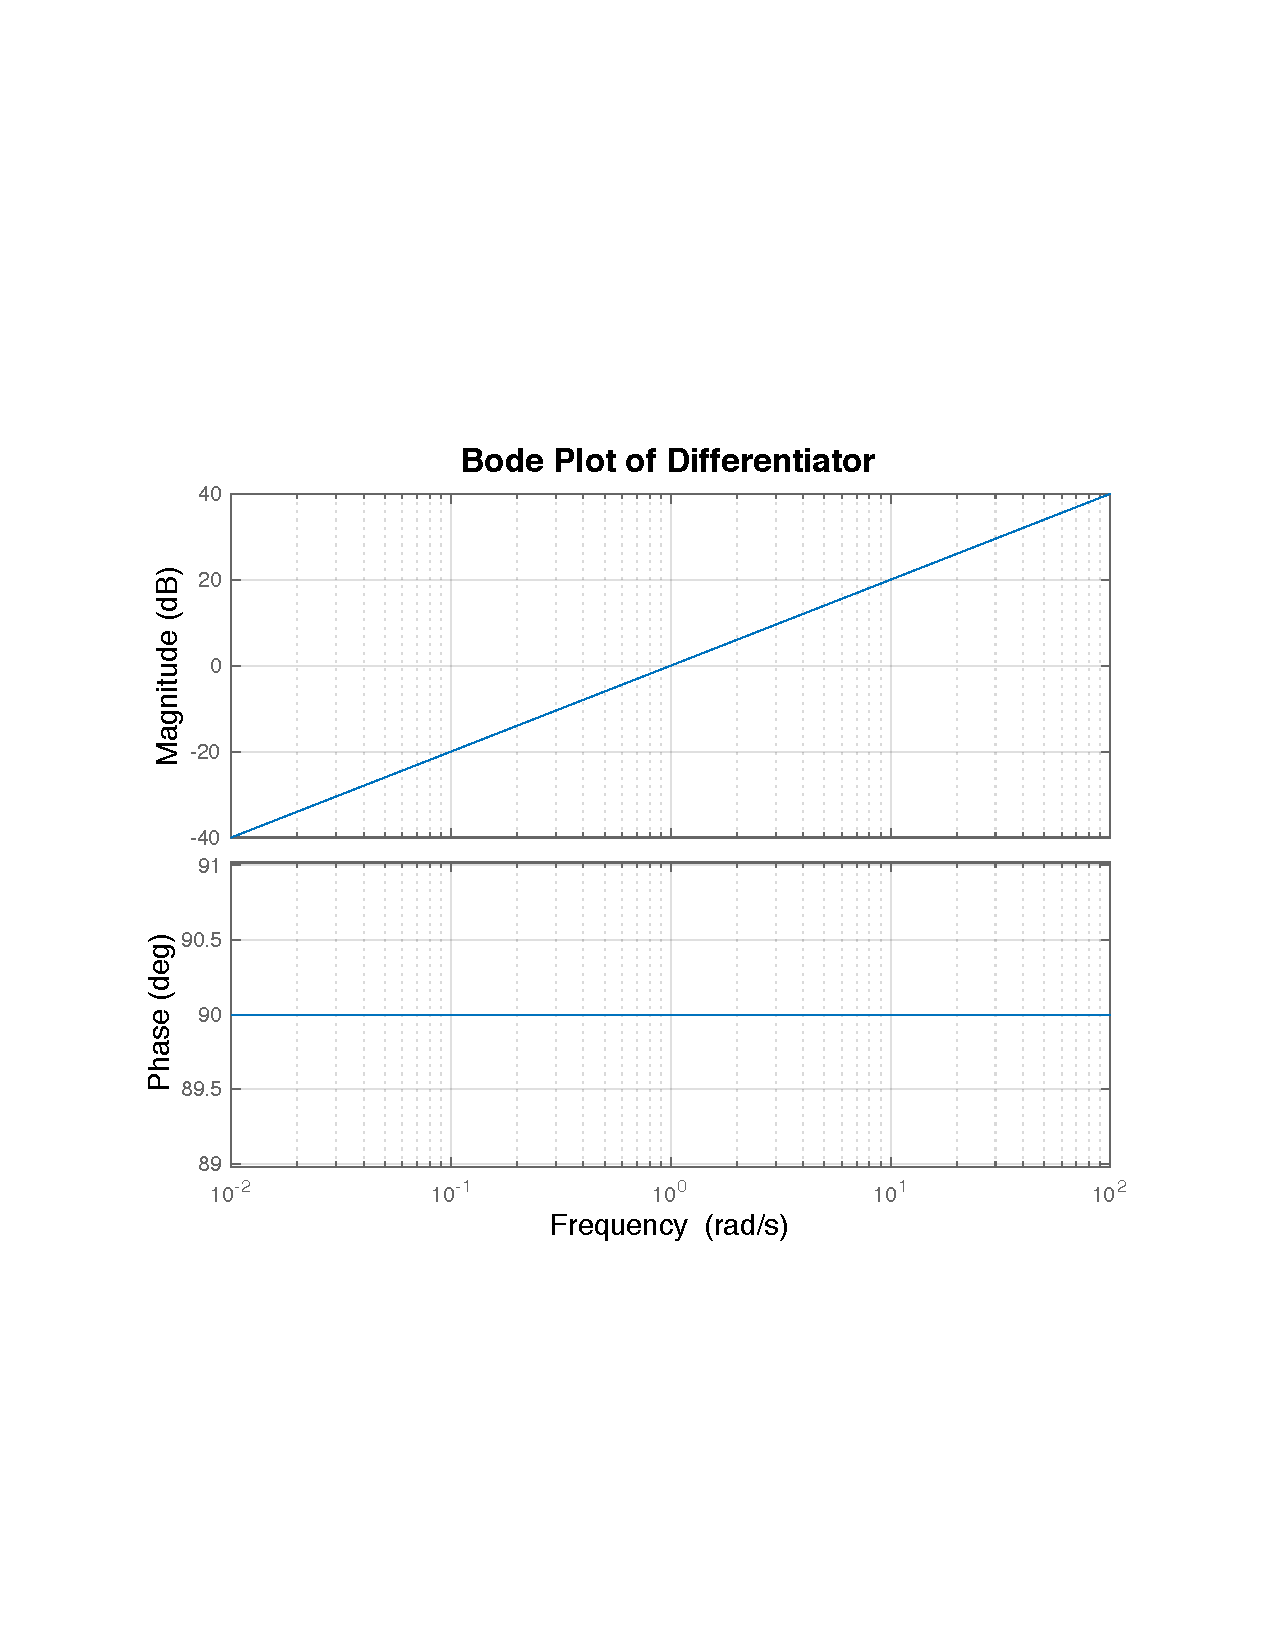
\includegraphics[width=0.8\linewidth]{figures/Differentiator.pdf}
\caption{Bode plot of differentiator.}
\label{fig_bode_differentiator}
\end{figure}



\section{Velocity and Distance Estimation using Kalman Filter}

i)


 A state space model is derived for estimation of velocity and distance based on accelerometer measurements. The states are position and velocity, while the input is the acceleration as shown in equation \ref{eq_input_states_simple}. Underline, $\underline{\cdot}$, denotes a vector.

\begin{align}
    u = \ddot{x}, \quad \quad \quad x_1 = x, \quad \quad \quad x_2 = \dot{x}_1 = \dot{x}, \quad \quad \quad \underline{x} = \begin{bmatrix}
    x_1 & x_2
    \end{bmatrix}
    ^T
    \label{eq_input_states_simple}
\end{align}

 The state and output equations, i.e. the state space model, are shown in equation \ref{eq_ss_simple}.


\begin{align}
    \underline{\dot{x}} = 
    \begin{bmatrix}
    0 & 1\\
    0 & 0
    \end{bmatrix}
    \, 
    \underline{x} +
    \begin{bmatrix}
    0\\
    1
    \end{bmatrix}
    \, u, \quad \quad \quad
    y =
    \begin{bmatrix}
    0 & 0
    \end{bmatrix}
    \,
    \underline{x}
    \label{eq_ss_simple}
\end{align}

 To check whether the system is completely observable, the observability matrix is calculated: KILDE

\begin{align}
    \underline{\mathcal{O}} =
    \begin{bmatrix}
    \underline{C}^T & (\underline{C}\,\underline{A})^T
    \end{bmatrix}
    =
    \begin{bmatrix}
    0 & 0 \\
    0 & 0 \\
    \end{bmatrix}
\end{align}

 The system is not observable as the determinant of the observability matrix is zero meaning the rows and columns are linear dependent. KILDE\\

 A new state space model is derived for estimation velocity and distance however now there is access to both accelerometer measurements and height measurements from the pressure sensor.\\

 The states and input remain the same but now there is a measured output $y$:

\begin{align}
    \underline{\dot{x}}= 
    \begin{bmatrix}
    0 & 1\\
    0 & 0
    \end{bmatrix}
    \, 
    \underline{x} +
    \begin{bmatrix}
    0\\
    1
    \end{bmatrix}
    \, u, \quad \quad \quad
    y =
    \begin{bmatrix}
    1 & 0
    \end{bmatrix}
    \,
    \underline{x} 
\end{align}


 The observability matrix is calculated in equation \ref{eq_observabi}.

\begin{align}
    \underline{\mathcal{O}} =
    \begin{bmatrix}
    \underline{C}^T & (\underline{C}\,\underline{A})^T
    \end{bmatrix}
    =
    \begin{bmatrix}
    1 & 0 \\
    0 & 1 \\
    \end{bmatrix}
    \label{eq_observabi}
\end{align}

 The determinant of the observability matrix in equation \ref{eq_observabi} is non-zero and the system is completely observable.



\subsection{Discretisation of Continuous Model}

The continuous state space model is discretised using Euler approximation. KILDE 

\begin{align}
    \underline{x}(k+1) &= \underline{A}_q \, \underline{x}(k) + \underline{B}_q \, u(k)\nonumber\\
    y(k) &= \underline{C}_q \, \underline{x}(k)
\end{align}

 Where:

\begin{align}
    \underline{A}_q = \underline{e}^{\underline{A} \, \Delta}, \quad \quad \quad \underline{B}_q = \int_0^\Delta \, \underline{e}^{\underline{A}\,(\Delta-\tau)} \, \underline{B} \, d\tau, \quad \quad \quad \underline{C}_q = \underline{C}
\end{align}

 $\Delta$ is the sampling period. The continuous-time state space model is discretised in equation \ref{eq_discretisation}.

\begin{align}
\underline{x}(k+1) &= 
\begin{bmatrix}
1 & \Delta\\
0 & 1
\end{bmatrix}
\,
\underline{x}(k) + 
\begin{bmatrix}
\frac{1}{2} \, \Delta^2\\
\Delta
\end{bmatrix}
\,
u(k) + w(k) \nonumber\\
 \nonumber\\
 \underline{y}(k) &=
\begin{bmatrix}
1 & 0 
\end{bmatrix}
\,
\underline{x}(k) + v(k)
    \label{eq_discretisation}
\end{align}

In equation \ref{eq_discretisation}, $w(k)$ and $v(k)$ are Gaussian white noise random processes representing model errors and measurement noise.

\begin{align}
    \dot{x} = A \, x + B \, u + w, \quad \quad \quad y = C \, x + v
\end{align}


\begin{align}
    \dot{\hat{x}} = A \, \hat{x} + B \, u + L(y - C \, \hat{x})
\end{align}

\begin{figure}[H]
\centering
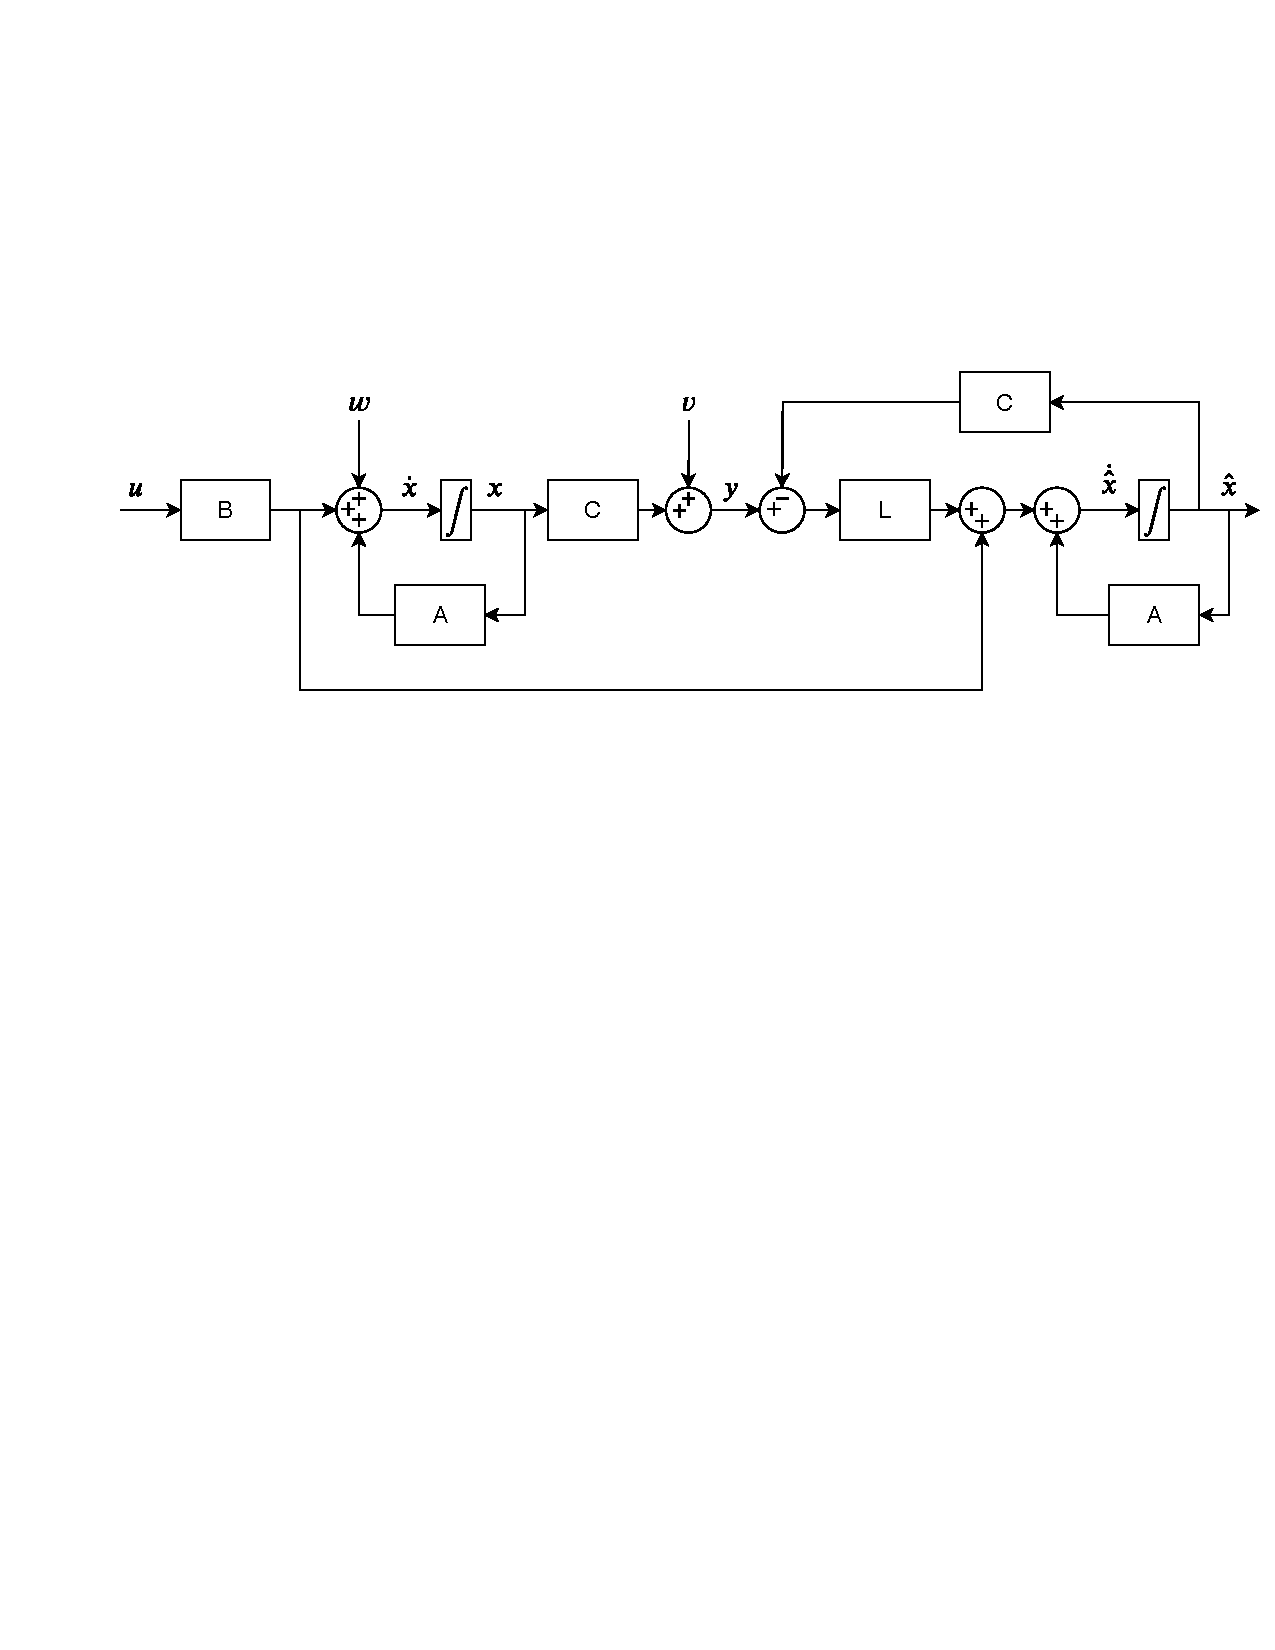
\includegraphics[width=\linewidth]{figures/ContinuousKalman.pdf}
\caption{Block diagram of system with Kalman filter.}
\label{fig_continuous_kalman}
\end{figure}


iii) 

\begin{align}
    \hat{x}_{k+1}^- &= A \, \hat{x}_k^+ + B \, u_k \nonumber\\
    P_{k+1}^- &= A\, P_k^+ \, A^T + Q_k
\end{align}

\begin{align}
    \hat{x}_k^+ &= \hat{x}_k^- + K_k (y_k - C \, \hat{x}_k^-)\nonumber\\
    K_k &= P_k^- \, C^T (R_k + C \,P_k^- \, C^T)^{-1}\nonumber\\
    P_k^+ &= (I -K_k \, C) P_k^-
\end{align}



\section{Distance Estimation using Kalman Filter in Real Time}

\section{Results and Discussion}



\bibliography{sample}

\end{document}